\documentclass[hyperref={pdfpagelabels=false}]{beamer}
\usepackage{lmodern}
\usetheme{CambridgeUS}
\title{\\Meccanismi che condizionano l'espressione genica\\}  
\author{\\ C. Bartalotta, D. Santilli e D. Bernardini} 
\date{\today} 
\begin{document}
\logo{
\includegraphics[scale=0.05]{logoRomaTre}}


\begin{frame}
\titlepage
\end{frame} 


\begin{frame}\frametitle{L'espressione Genica}
\textbf{Espressione genica:}\\
processo grazie al quale l'informazione contenuta in un gene viene convertita in una macromolecola funzionale.
\'E un processo a pi\'u stadi:\pause 
\begin{enumerate}
\item trascrizione del DNA in RNA:\\
produzione dell'RNA complementare a una delle due eliche del gene  \pause 
\item maturazione:\\
l'RNA trascritto puo' essere modificato (maturazione) per dare origine a quello che si chiama RNA (funzionante) maturo \pause 
\item traduzione:\\
l'RNA messaggero o mRNA viene tradotto nella proteina corrispondente
\end{enumerate}
\end{frame}


\begin{frame}\frametitle{Controllo dell'espressione genica}
L'evoluzione ha consentito che le funzioni cellulari si accendano e spengano a seconda del loro effettivo bisogno. Questo fa si che le cellule si differenzino al fine di svolgere ruoli specializzati.
\\
Due tipi di gene:
\begin{itemize}
\item \textbf{Geni regolati:} la trascrizione e la traduzione sono sotto stretto controllo cellulare per far si che la quantit\'a del loro prodotto (proteina o RNA) sia controllata in base al fabbisogno cellulare. I geni regolati sono quindi espressi solo in alcuni tipi di cellule e solo in determinati momenti, in risposta a determinati stimoli.
\item \textbf{Geni costitutivi:} costantemente attivi perch\'e essenziali per svolegere i processi di base. Questo tipo di gene, anche chiamato \emph{housekeeping genes}, viene continuamente trascritto in quanto codifica proteine necessarie per il mantenimento di funzioni generali. Essi sono riconosciuti da attivatori  presenti in tutte le 
cellule.
\end{itemize}
\end{frame}


\begin{frame}\frametitle{Regolazione dell'espressione genica}
La regolazione pu\'o avvenire a diversi livelli:
\begin{block}{Livello di trascrizione}
Le proteine regolatrici, attivatori o repressori, interagiscono con il DNA ed in base ai cambiamenti ambientali attivano o disattivano i geni. A questo livello, il controllo stabilisce quali geni vengono trascritti e per quanto tempo.
\end{block}
\begin{block}{Livello di maturazione}
I controlli a livello di maturazione agiscono determinando quali parti dei trascritti primari entrano a far parte degli mRNA cellulari.
\end{block}
\begin{block}{Livello di traduzione}
I controlli a livello di traduzione determinano se un mRNA deve essere tradotto, per quanto tempo e quanto frequentemente.
\end{block}
\end{frame}


\begin{frame}\frametitle{Controllo prima della trascrizione}
 Prima che un gene venga trascritto in mRNA, la regolazione genica pu\'o avvenire mediante una modifica della struttura della cromatina.\\
 La cromatina pu\'o essere infatti di due tipi: \textbf{eucromatina} e \textbf{eterocromatina}. La prima corrisponde al DNA che viene trascritto in RNA, la seconda , al contrario, contiene geni che non vengono trascritti.
 Modificando quindi la struttura della cromatina, \'e possibile impedire che l' RNA polimerasi e le proteine si leghino per iniziare il processo di trascrizione.
\end{frame}


\begin{frame} \frametitle{Controllo a livello della trascrizione}
Questo livello di regolazione costituisce un ruolo fondamentale in quanto, determinando quali geni devono essere attivati o spenti, si stabilisce anche quali proteine verranno sintetizzate nell'arco di vita cellulare.\\
La trascrizione diferenziale avviene grazie determinate sequenze di DNA e proteine:
\begin{itemize}
\item \textbf{sequenze regolatrici} alle quali si legano le proteine regolatrici che attivano il processo di trascrizione.
\item \textbf{sequenze amplificatrici} alle qualisi legano \emph{proteine attivatrici} che stimolano il processo di trascrizione.
\item \textbf{sequenze silenziatrici} alle quali si legano le \emph{proteine repressori} che inibiscono la trascrizione.
\end{itemize}
\end{frame}


\begin{frame}\frametitle{Sequenza proteica}
\centering 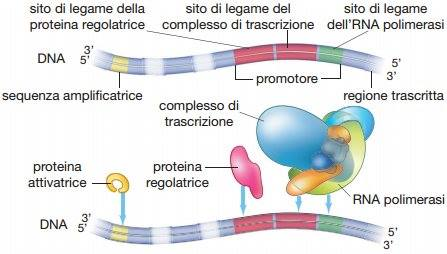
\includegraphics[width=8cm,height=4cm]{sequenzeProteine.jpg}
\end{frame}


\begin{frame}\frametitle{Sequenza amplificatrice}
\begin{minipage}[c]{.45\textwidth}
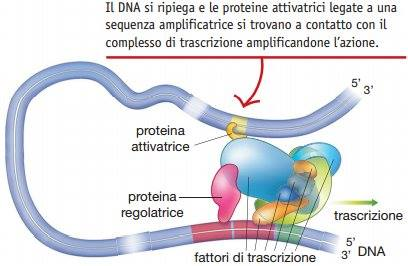
\includegraphics[width=5cm,height=4cm]{proteine.jpg}
\end{minipage}
\begin{minipage}[c]{.5\textwidth}
Al fine di produrre una quantit\'a maggiore di una determinata proteina, rispetto ad un'altra, le cellule ricorrono all' \emph{amplificazione genica}. In questo modo vengono prodotte pi\'u copie dello stesso gene che vengono poi tutte trascritte.
\end{minipage}
\end{frame}


\begin{frame}\frametitle{Controllo dopo la trascrizione (Maturazione)}
In generale, i geni sono costituiti da \textbf{introni}, sequenze di nucleotidi non codificanti e da \textbf{esoni}, tratti codificanti. Un gene cos\'i formato viene definito \textbf{gene interrotto}.\\
Quando un gene interrotto viene trascritto, il corrispondente pre-mRNA contiene anche gli introni. Durante il processo di maturazione, attraverso lo \textbf{splicing dell'RNA}, vengono tagliati gli introni e congiunti gli esoni.\\
Attraverso lo \textbf{splicing alternativo}, \'e possibile regolare l'espressione genica tagliando anche sequenze di \emph{esoni} oltra agli introni.
\end{frame}


\begin{frame}\frametitle{Controllo a livello di traduzione}
La longevit\'a di traduzione dell' mRNA \'e dettata dall'\textbf{emivita}, il tempo affinche il 50\% delle proteine prese in considerazione vengano degradate.\\
La sintesi delle proteine pu\'o avvenire molto rapidamente perch\'e pi\'u ribosomi possono legarsi ad uno stesso filamento di mRNA consentendo quindi la costruzione simultanea di pi\'u catene proteiche.
\begin{minipage}[c]{.5\textwidth}
Il \textbf{ribosoma} rappresenta la macchina esecutrice della sintesi proteica, composto per i 2/3 da RNA e per 1/3 da proteine.\\
Il \textbf{tRNA} \'e una piccola catena di RNA che trasferisce un amminoacido specifico di una catena polipeptidica in crescita al sito ribosomiale.
\end{minipage}
\begin{minipage}[c]{.45\textwidth}
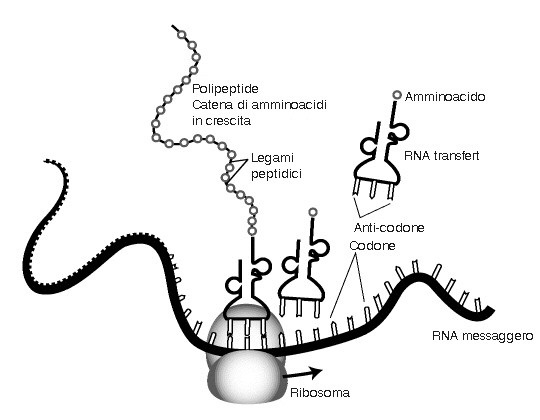
\includegraphics[width=5cm,height=4cm]{traduzione.jpg}
\end{minipage}
\end{frame}


\begin{frame}\frametitle{Considerazioni finali}
Se vogliamo scriviamo qualcosa, altrimenti per me va bene com'\'e ora..
\end{frame}


\end{document}